\subsection{Simulation RANS}

L'approche RANS utilisent un opérateur de moyenne statistique(add ref ). Les equation obtenue à l'aide des opérateurs est un systeme d'équation ouvert. Plusieurs modéle de turbulence permettent de fermé le systeme d'equation RANS. Les plus connus sont les modéles k-omega sst de Mender[ref], le modele spalart allmaras de P.R. Spalart (ref)et le modele k epesilon de Jones, W. P., and Launder, B. E. (1972).\\
Les calculs RANS reposent sur des equatons moyenné et génerent donc des champs d'écoulement moyen. Cette Methode est le plus souvent utilisé pour des calculs stationnaires. Ils sont tres utilisé dans le monde de l'industrie des calculs turbulent pour sont cout de calculs qui est tres interresant.\\
Cependant en moyennant les variables turbulente il est imossible de calculer les fluctuations de ces varaibles au cours du temps à contrario des autres methodes. Comme représenté sur la figure (ref fig) lors de dimensionnment d'enjin spaciaux il est crucial d'obtenir des fluctuations au cours du temps, pour la pression ou la temperature. Si lors d'une rentré atmopherique, les materiuax d'une vehicule atteignent une température de fusion, le matériaux sera dégradé et cela pourra enjendrer des consequances terribles lors d' une mission.

\begin{figure}[h!]
 \centering
 \includegraphics[width=0.7\linewidth]{chapter1_introduction/pictures/les_rans_dns.png}
 \vspace{-2ex}
 \caption{IXV spatial navette by esa}
  \vspace{2ex}
 \label{rans}
\end{figure}
